% Options for packages loaded elsewhere
\PassOptionsToPackage{unicode}{hyperref}
\PassOptionsToPackage{hyphens}{url}
\PassOptionsToPackage{dvipsnames,svgnames,x11names}{xcolor}
%
\documentclass[
  letterpaper,
  DIV=11,
  numbers=noendperiod]{scrartcl}

\usepackage{amsmath,amssymb}
\usepackage{iftex}
\ifPDFTeX
  \usepackage[T1]{fontenc}
  \usepackage[utf8]{inputenc}
  \usepackage{textcomp} % provide euro and other symbols
\else % if luatex or xetex
  \usepackage{unicode-math}
  \defaultfontfeatures{Scale=MatchLowercase}
  \defaultfontfeatures[\rmfamily]{Ligatures=TeX,Scale=1}
\fi
\usepackage{lmodern}
\ifPDFTeX\else  
    % xetex/luatex font selection
\fi
% Use upquote if available, for straight quotes in verbatim environments
\IfFileExists{upquote.sty}{\usepackage{upquote}}{}
\IfFileExists{microtype.sty}{% use microtype if available
  \usepackage[]{microtype}
  \UseMicrotypeSet[protrusion]{basicmath} % disable protrusion for tt fonts
}{}
\makeatletter
\@ifundefined{KOMAClassName}{% if non-KOMA class
  \IfFileExists{parskip.sty}{%
    \usepackage{parskip}
  }{% else
    \setlength{\parindent}{0pt}
    \setlength{\parskip}{6pt plus 2pt minus 1pt}}
}{% if KOMA class
  \KOMAoptions{parskip=half}}
\makeatother
\usepackage{xcolor}
\setlength{\emergencystretch}{3em} % prevent overfull lines
\setcounter{secnumdepth}{-\maxdimen} % remove section numbering
% Make \paragraph and \subparagraph free-standing
\makeatletter
\ifx\paragraph\undefined\else
  \let\oldparagraph\paragraph
  \renewcommand{\paragraph}{
    \@ifstar
      \xxxParagraphStar
      \xxxParagraphNoStar
  }
  \newcommand{\xxxParagraphStar}[1]{\oldparagraph*{#1}\mbox{}}
  \newcommand{\xxxParagraphNoStar}[1]{\oldparagraph{#1}\mbox{}}
\fi
\ifx\subparagraph\undefined\else
  \let\oldsubparagraph\subparagraph
  \renewcommand{\subparagraph}{
    \@ifstar
      \xxxSubParagraphStar
      \xxxSubParagraphNoStar
  }
  \newcommand{\xxxSubParagraphStar}[1]{\oldsubparagraph*{#1}\mbox{}}
  \newcommand{\xxxSubParagraphNoStar}[1]{\oldsubparagraph{#1}\mbox{}}
\fi
\makeatother

\usepackage{color}
\usepackage{fancyvrb}
\newcommand{\VerbBar}{|}
\newcommand{\VERB}{\Verb[commandchars=\\\{\}]}
\DefineVerbatimEnvironment{Highlighting}{Verbatim}{commandchars=\\\{\}}
% Add ',fontsize=\small' for more characters per line
\usepackage{framed}
\definecolor{shadecolor}{RGB}{241,243,245}
\newenvironment{Shaded}{\begin{snugshade}}{\end{snugshade}}
\newcommand{\AlertTok}[1]{\textcolor[rgb]{0.68,0.00,0.00}{#1}}
\newcommand{\AnnotationTok}[1]{\textcolor[rgb]{0.37,0.37,0.37}{#1}}
\newcommand{\AttributeTok}[1]{\textcolor[rgb]{0.40,0.45,0.13}{#1}}
\newcommand{\BaseNTok}[1]{\textcolor[rgb]{0.68,0.00,0.00}{#1}}
\newcommand{\BuiltInTok}[1]{\textcolor[rgb]{0.00,0.23,0.31}{#1}}
\newcommand{\CharTok}[1]{\textcolor[rgb]{0.13,0.47,0.30}{#1}}
\newcommand{\CommentTok}[1]{\textcolor[rgb]{0.37,0.37,0.37}{#1}}
\newcommand{\CommentVarTok}[1]{\textcolor[rgb]{0.37,0.37,0.37}{\textit{#1}}}
\newcommand{\ConstantTok}[1]{\textcolor[rgb]{0.56,0.35,0.01}{#1}}
\newcommand{\ControlFlowTok}[1]{\textcolor[rgb]{0.00,0.23,0.31}{\textbf{#1}}}
\newcommand{\DataTypeTok}[1]{\textcolor[rgb]{0.68,0.00,0.00}{#1}}
\newcommand{\DecValTok}[1]{\textcolor[rgb]{0.68,0.00,0.00}{#1}}
\newcommand{\DocumentationTok}[1]{\textcolor[rgb]{0.37,0.37,0.37}{\textit{#1}}}
\newcommand{\ErrorTok}[1]{\textcolor[rgb]{0.68,0.00,0.00}{#1}}
\newcommand{\ExtensionTok}[1]{\textcolor[rgb]{0.00,0.23,0.31}{#1}}
\newcommand{\FloatTok}[1]{\textcolor[rgb]{0.68,0.00,0.00}{#1}}
\newcommand{\FunctionTok}[1]{\textcolor[rgb]{0.28,0.35,0.67}{#1}}
\newcommand{\ImportTok}[1]{\textcolor[rgb]{0.00,0.46,0.62}{#1}}
\newcommand{\InformationTok}[1]{\textcolor[rgb]{0.37,0.37,0.37}{#1}}
\newcommand{\KeywordTok}[1]{\textcolor[rgb]{0.00,0.23,0.31}{\textbf{#1}}}
\newcommand{\NormalTok}[1]{\textcolor[rgb]{0.00,0.23,0.31}{#1}}
\newcommand{\OperatorTok}[1]{\textcolor[rgb]{0.37,0.37,0.37}{#1}}
\newcommand{\OtherTok}[1]{\textcolor[rgb]{0.00,0.23,0.31}{#1}}
\newcommand{\PreprocessorTok}[1]{\textcolor[rgb]{0.68,0.00,0.00}{#1}}
\newcommand{\RegionMarkerTok}[1]{\textcolor[rgb]{0.00,0.23,0.31}{#1}}
\newcommand{\SpecialCharTok}[1]{\textcolor[rgb]{0.37,0.37,0.37}{#1}}
\newcommand{\SpecialStringTok}[1]{\textcolor[rgb]{0.13,0.47,0.30}{#1}}
\newcommand{\StringTok}[1]{\textcolor[rgb]{0.13,0.47,0.30}{#1}}
\newcommand{\VariableTok}[1]{\textcolor[rgb]{0.07,0.07,0.07}{#1}}
\newcommand{\VerbatimStringTok}[1]{\textcolor[rgb]{0.13,0.47,0.30}{#1}}
\newcommand{\WarningTok}[1]{\textcolor[rgb]{0.37,0.37,0.37}{\textit{#1}}}

\providecommand{\tightlist}{%
  \setlength{\itemsep}{0pt}\setlength{\parskip}{0pt}}\usepackage{longtable,booktabs,array}
\usepackage{calc} % for calculating minipage widths
% Correct order of tables after \paragraph or \subparagraph
\usepackage{etoolbox}
\makeatletter
\patchcmd\longtable{\par}{\if@noskipsec\mbox{}\fi\par}{}{}
\makeatother
% Allow footnotes in longtable head/foot
\IfFileExists{footnotehyper.sty}{\usepackage{footnotehyper}}{\usepackage{footnote}}
\makesavenoteenv{longtable}
\usepackage{graphicx}
\makeatletter
\def\maxwidth{\ifdim\Gin@nat@width>\linewidth\linewidth\else\Gin@nat@width\fi}
\def\maxheight{\ifdim\Gin@nat@height>\textheight\textheight\else\Gin@nat@height\fi}
\makeatother
% Scale images if necessary, so that they will not overflow the page
% margins by default, and it is still possible to overwrite the defaults
% using explicit options in \includegraphics[width, height, ...]{}
\setkeys{Gin}{width=\maxwidth,height=\maxheight,keepaspectratio}
% Set default figure placement to htbp
\makeatletter
\def\fps@figure{htbp}
\makeatother

\usepackage{booktabs}
\usepackage{longtable}
\usepackage{array}
\usepackage{multirow}
\usepackage{wrapfig}
\usepackage{float}
\usepackage{colortbl}
\usepackage{pdflscape}
\usepackage{tabu}
\usepackage{threeparttable}
\usepackage{threeparttablex}
\usepackage[normalem]{ulem}
\usepackage{makecell}
\usepackage{xcolor}
\KOMAoption{captions}{tableheading}
\makeatletter
\@ifpackageloaded{caption}{}{\usepackage{caption}}
\AtBeginDocument{%
\ifdefined\contentsname
  \renewcommand*\contentsname{Table of contents}
\else
  \newcommand\contentsname{Table of contents}
\fi
\ifdefined\listfigurename
  \renewcommand*\listfigurename{List of Figures}
\else
  \newcommand\listfigurename{List of Figures}
\fi
\ifdefined\listtablename
  \renewcommand*\listtablename{List of Tables}
\else
  \newcommand\listtablename{List of Tables}
\fi
\ifdefined\figurename
  \renewcommand*\figurename{Figure}
\else
  \newcommand\figurename{Figure}
\fi
\ifdefined\tablename
  \renewcommand*\tablename{Table}
\else
  \newcommand\tablename{Table}
\fi
}
\@ifpackageloaded{float}{}{\usepackage{float}}
\floatstyle{ruled}
\@ifundefined{c@chapter}{\newfloat{codelisting}{h}{lop}}{\newfloat{codelisting}{h}{lop}[chapter]}
\floatname{codelisting}{Listing}
\newcommand*\listoflistings{\listof{codelisting}{List of Listings}}
\makeatother
\makeatletter
\makeatother
\makeatletter
\@ifpackageloaded{caption}{}{\usepackage{caption}}
\@ifpackageloaded{subcaption}{}{\usepackage{subcaption}}
\makeatother

\ifLuaTeX
  \usepackage{selnolig}  % disable illegal ligatures
\fi
\usepackage{bookmark}

\IfFileExists{xurl.sty}{\usepackage{xurl}}{} % add URL line breaks if available
\urlstyle{same} % disable monospaced font for URLs
\hypersetup{
  pdftitle={Report on Diabetes Behavioral Factors Analysis},
  pdfauthor={Anupama Bishwokarma},
  colorlinks=true,
  linkcolor={blue},
  filecolor={Maroon},
  citecolor={Blue},
  urlcolor={Blue},
  pdfcreator={LaTeX via pandoc}}


\title{Report on Diabetes Behavioral Factors Analysis}
\author{Anupama Bishwokarma}
\date{}

\begin{document}
\maketitle


\subsection{Project overview}\label{project-overview}

Diabetes behavioral factors analysis project analyzes the responses
collected among the adults in the United States using Behavioral Risk
Factor Surveillance System (BRFSS) in 2023. The project is using on R
programming language.

\subsection{Project objectives}\label{project-objectives}

\begin{enumerate}
\def\labelenumi{\arabic{enumi}.}
\tightlist
\item
  To explore the socio-demographic, biological and behavioral
  characteristics of the respondents
\item
  To examine the association of behavioral factors with the diabetes
  status
\end{enumerate}

\subsection{BRFSS dataset overview}\label{brfss-dataset-overview}

BRFSS collects uniform state-specific data on health risk behaviors,
chronic diseases and conditions, access to health care, and use of
preventive health services related to the leading causes of death and
disability in the United States. Data Source:
\url{https://www.cdc.gov/brfss/annual_data/annual_2023.html} under the
file name {[}2023 BRFSS Data (SAS Transport Format){]}.

\begin{Shaded}
\begin{Highlighting}[]
\CommentTok{\# Load dataset}
\NormalTok{whole\_brfss }\OtherTok{\textless{}{-}} \FunctionTok{readRDS}\NormalTok{(}\StringTok{"01\_Datasets/whole\_BRFSS\_2023.rds"}\NormalTok{)}
\end{Highlighting}
\end{Shaded}

\subsection{Data preparation: subsetting, labelling, recoding,
standardizing}\label{data-preparation-subsetting-labelling-recoding-standardizing}

The loaded dataset was explored for relevant variables for the project.
Additionally, I referred to questionnaire
\url{https://www.cdc.gov/brfss/questionnaires/pdf-ques/2023-BRFSS-Questionnaire-508.pdf}
used for the survey to understand the topic and questions. The whole
dataset included 350 variables with 400,000+ rows.

The dataset was filtered for the relevant 12 variables with same number
of observations. These variables included: socio-demographic,
biological, behavioral and diabetes related variables. The outcome
variable is of ``Diabetes Status''.

Then, the selected variables were renamed for easy readability.

\begin{Shaded}
\begin{Highlighting}[]
\CommentTok{\# Renaming the variables: }
\FunctionTok{names}\NormalTok{(short\_brfss) }\OtherTok{\textless{}{-}} \FunctionTok{c}\NormalTok{(}\StringTok{"id\_no"}\NormalTok{, }
                        \StringTok{"state\_name"}\NormalTok{,        }\CommentTok{\# Name of the State}
                        \StringTok{"age"}\NormalTok{,               }\CommentTok{\# Age of the respondent}
                        \StringTok{"sex"}\NormalTok{,               }\CommentTok{\# Sex of the respondent}
                        \StringTok{"income\_level"}\NormalTok{,      }\CommentTok{\# Annual Household income from all sources}
                        \StringTok{"BMI"}\NormalTok{,               }\CommentTok{\# Body Mass Index}
                        \StringTok{"physical\_activity"}\NormalTok{, }\CommentTok{\# Any physical activity in past month?}
                        \StringTok{"smoking"}\NormalTok{,           }\CommentTok{\# Current smoking status}
                        \StringTok{"tobacco\_use"}\NormalTok{,       }\CommentTok{\# Current tobacco use}
                        \StringTok{"alc\_drnk\_30days"}\NormalTok{,   }\CommentTok{\# At least one drink of alcohol in the past 30 days}
                        \StringTok{"diabetes\_status"}\NormalTok{,   }\CommentTok{\# Diabetes status}
                        \StringTok{"diab\_first\_known"}\NormalTok{)  }\CommentTok{\# Age when first told had diabetes}
\end{Highlighting}
\end{Shaded}

Next, dataset was checked for the type of variables. The dataset
included of numeric and character data types. Categorical variables were
integer-encoded.

Following this, categorical variables were converted to labeled factors.
The levels ``Yes'' and ``No'' of ``smoking'' were reordered for
uniformity. Additionally, levels of certain variables (e.g,
``tobacco\_use'', ``diabetes\_status'' ) were re-classified to
two-levels.

\begin{Shaded}
\begin{Highlighting}[]
\CommentTok{\# assign labels to variable: state\_name}
\NormalTok{state\_labels }\OtherTok{\textless{}{-}} \FunctionTok{c}\NormalTok{(}\StringTok{"1"} \OtherTok{=} \StringTok{"Alabama"}\NormalTok{, }\StringTok{"2"} \OtherTok{=} \StringTok{"Alaska"}\NormalTok{, }\StringTok{"4"} \OtherTok{=} \StringTok{"Arizona"}\NormalTok{, }
                  \StringTok{"5"} \OtherTok{=} \StringTok{"Arkansas"}\NormalTok{, }\StringTok{"6"} \OtherTok{=} \StringTok{"California"}\NormalTok{, }\StringTok{"8"} \OtherTok{=} \StringTok{"Colorado"}\NormalTok{, }
                  \StringTok{"9"} \OtherTok{=} \StringTok{"Connecticut"}\NormalTok{, }\StringTok{"10"} \OtherTok{=} \StringTok{"Delaware"}\NormalTok{, }
                  \StringTok{"11"} \OtherTok{=} \StringTok{"District of Columbia"}\NormalTok{, }\StringTok{"12"} \OtherTok{=} \StringTok{"Florida"}\NormalTok{, }
                  \StringTok{"13"} \OtherTok{=} \StringTok{"Georgia"}\NormalTok{, }\StringTok{"15"} \OtherTok{=} \StringTok{"Hawaii"}\NormalTok{, }\StringTok{"16"} \OtherTok{=} \StringTok{"Idaho"}\NormalTok{, }
                  \StringTok{"17"} \OtherTok{=} \StringTok{"Illinois"}\NormalTok{, }\StringTok{"18"} \OtherTok{=} \StringTok{"Indiana"}\NormalTok{, }\StringTok{"19"} \OtherTok{=} \StringTok{"Iowa"}\NormalTok{, }
                  \StringTok{"20"} \OtherTok{=} \StringTok{"Kansas"}\NormalTok{, }\StringTok{"22"} \OtherTok{=} \StringTok{"Louisiana"}\NormalTok{, }\StringTok{"23"} \OtherTok{=} \StringTok{"Maine"}\NormalTok{, }
                  \StringTok{"24"} \OtherTok{=} \StringTok{"Maryland"}\NormalTok{, }\StringTok{"25"} \OtherTok{=} \StringTok{"Massachusetts"}\NormalTok{, }\StringTok{"26"} \OtherTok{=} \StringTok{"Michigan"}\NormalTok{,}
                  \StringTok{"27"} \OtherTok{=} \StringTok{"Minnesota"}\NormalTok{, }\StringTok{"28"} \OtherTok{=} \StringTok{"Mississippi"}\NormalTok{, }\StringTok{"29"} \OtherTok{=} \StringTok{"Missouri"}\NormalTok{, }
                  \StringTok{"30"} \OtherTok{=} \StringTok{"Montana"}\NormalTok{, }\StringTok{"31"} \OtherTok{=} \StringTok{"Nebraska"}\NormalTok{, }\StringTok{"32"} \OtherTok{=} \StringTok{"Nevada"}\NormalTok{, }
                  \StringTok{"33"} \OtherTok{=} \StringTok{"New Hampshire"}\NormalTok{, }\StringTok{"34"} \OtherTok{=} \StringTok{"New Jersey"}\NormalTok{, }
                  \StringTok{"35"} \OtherTok{=} \StringTok{"New Mexico"}\NormalTok{, }\StringTok{"36"} \OtherTok{=} \StringTok{"New York"}\NormalTok{, }\StringTok{"37"} \OtherTok{=} \StringTok{"North Carolina"}\NormalTok{,}
                  \StringTok{"38"} \OtherTok{=} \StringTok{"North Dakota"}\NormalTok{, }\StringTok{"39"} \OtherTok{=} \StringTok{"Ohio"}\NormalTok{, }\StringTok{"40"} \OtherTok{=} \StringTok{"Oklahoma"}\NormalTok{, }
                  \StringTok{"41"} \OtherTok{=} \StringTok{"Oregon"}\NormalTok{, }\StringTok{"44"} \OtherTok{=} \StringTok{"Rhode Island"}\NormalTok{, }
                  \StringTok{"45"} \OtherTok{=} \StringTok{"South Carolina"}\NormalTok{, }\StringTok{"46"} \OtherTok{=} \StringTok{"South Dakota"}\NormalTok{, }
                  \StringTok{"47"} \OtherTok{=} \StringTok{"Tennessee"}\NormalTok{, }\StringTok{"48"} \OtherTok{=} \StringTok{"Texas"}\NormalTok{, }\StringTok{"49"} \OtherTok{=} \StringTok{"Utah"}\NormalTok{, }
                  \StringTok{"50"} \OtherTok{=} \StringTok{"Vermont"}\NormalTok{, }\StringTok{"51"} \OtherTok{=} \StringTok{"Virginia"}\NormalTok{, }\StringTok{"53"} \OtherTok{=} \StringTok{"Washington"}\NormalTok{, }
                  \StringTok{"54"} \OtherTok{=} \StringTok{"West Virginia"}\NormalTok{, }\StringTok{"55"} \OtherTok{=} \StringTok{"Wisconsin"}\NormalTok{, }\StringTok{"56"} \OtherTok{=} \StringTok{"Wyoming"}\NormalTok{, }
                  \StringTok{"66"} \OtherTok{=} \StringTok{"Guam"}\NormalTok{, }\StringTok{"72"} \OtherTok{=} \StringTok{"Puerto Rico"}\NormalTok{, }\StringTok{"78"} \OtherTok{=} \StringTok{"Virgin Islands"}
\NormalTok{                  )}


\NormalTok{short\_brfss}\SpecialCharTok{$}\NormalTok{state\_name }\OtherTok{\textless{}{-}} \FunctionTok{factor}\NormalTok{(short\_brfss}\SpecialCharTok{$}\NormalTok{state\_name,}
                                 \AttributeTok{levels =} \FunctionTok{as.numeric}\NormalTok{(}\FunctionTok{names}\NormalTok{(state\_labels)),}
                                 \AttributeTok{labels =}\NormalTok{ state\_labels}
\NormalTok{                                 )}


\CommentTok{\# assign labels to variable: sex}
\NormalTok{short\_brfss}\SpecialCharTok{$}\NormalTok{sex }\OtherTok{\textless{}{-}} \FunctionTok{factor}\NormalTok{(short\_brfss}\SpecialCharTok{$}\NormalTok{sex, }
                              \AttributeTok{levels =} \FunctionTok{c}\NormalTok{(}\DecValTok{1}\NormalTok{, }\DecValTok{2}\NormalTok{),}
                              \AttributeTok{labels =} \FunctionTok{c}\NormalTok{(}\StringTok{"Male"}\NormalTok{, }\StringTok{"Female"}\NormalTok{))}


\CommentTok{\# assign labels to variable: income\_level}
\NormalTok{income\_labs }\OtherTok{\textless{}{-}} \FunctionTok{c}\NormalTok{(}\StringTok{"1"} \OtherTok{=} \StringTok{"Less than $15,000"}\NormalTok{,}
                         \StringTok{"2"} \OtherTok{=} \StringTok{"$15,000 to \textless{} $25,000"}\NormalTok{,}
                         \StringTok{"3"} \OtherTok{=} \StringTok{"$25,000 to \textless{} $35,000"}\NormalTok{,}
                         \StringTok{"4"} \OtherTok{=} \StringTok{"$35,000 to \textless{} $50,000"}\NormalTok{,}
                         \StringTok{"5"} \OtherTok{=} \StringTok{"$50,000 to \textless{} $100,000"}\NormalTok{,}
                         \StringTok{"6"} \OtherTok{=} \StringTok{"$100,000 to \textless{} $200,000"}\NormalTok{,}
                         \StringTok{"7"} \OtherTok{=} \StringTok{"$200,000 or more"}\NormalTok{,}
                         \StringTok{"9"} \OtherTok{=} \StringTok{"Don\textquotesingle{}t know/Not sure/Missing"}\NormalTok{)}


\NormalTok{short\_brfss}\SpecialCharTok{$}\NormalTok{income\_level}\OtherTok{\textless{}{-}} \FunctionTok{factor}\NormalTok{(short\_brfss}\SpecialCharTok{$}\NormalTok{income\_level,}
                                  \AttributeTok{levels =} \FunctionTok{as.numeric}\NormalTok{(}\FunctionTok{names}\NormalTok{(income\_labs)),}
                                  \AttributeTok{labels =}\NormalTok{ income\_labs)}


\CommentTok{\# assign labels to variable: physical\_activity}
\NormalTok{short\_brfss}\SpecialCharTok{$}\NormalTok{physical\_activity }\OtherTok{\textless{}{-}} \FunctionTok{factor}\NormalTok{(short\_brfss}\SpecialCharTok{$}\NormalTok{physical\_activity,}
                                            \AttributeTok{levels =} \FunctionTok{c}\NormalTok{(}\DecValTok{1}\NormalTok{, }\DecValTok{2}\NormalTok{, }\DecValTok{7}\NormalTok{, }\DecValTok{9}\NormalTok{),}
                                            \AttributeTok{labels =} \FunctionTok{c}\NormalTok{(}\StringTok{"Yes"}\NormalTok{,}
                                                       \StringTok{"No"}\NormalTok{,}
                                                       \StringTok{"Don\textquotesingle{}t know/Not Sure"}\NormalTok{,}
                                                       \StringTok{"Refused"}\NormalTok{))}


\CommentTok{\# assign labels to variable: smoking}
\NormalTok{short\_brfss}\SpecialCharTok{$}\NormalTok{smoking }\OtherTok{\textless{}{-}} \FunctionTok{factor}\NormalTok{(short\_brfss}\SpecialCharTok{$}\NormalTok{smoking,}
                                      \AttributeTok{levels =} \FunctionTok{c}\NormalTok{(}\DecValTok{1}\NormalTok{, }\DecValTok{2}\NormalTok{, }\DecValTok{9}\NormalTok{),}
                                      \AttributeTok{labels =} \FunctionTok{c}\NormalTok{(}\StringTok{"No"}\NormalTok{,}
                                                 \StringTok{"Yes"}\NormalTok{,}
                                                 \StringTok{"Don\textquotesingle{}t know/Refused/Missing"}\NormalTok{))}


\CommentTok{\#Reorder the levels of smoking}
\NormalTok{short\_brfss}\SpecialCharTok{$}\NormalTok{smoking }\OtherTok{\textless{}{-}} \FunctionTok{factor}\NormalTok{(short\_brfss}\SpecialCharTok{$}\NormalTok{smoking, }\AttributeTok{levels =} \FunctionTok{c}\NormalTok{(}\StringTok{"Yes"}\NormalTok{, }\StringTok{"No"}\NormalTok{))}



\CommentTok{\# assign labels to variable: tobacco\_use}
\NormalTok{short\_brfss}\SpecialCharTok{$}\NormalTok{tobacco\_use }\OtherTok{\textless{}{-}} \FunctionTok{factor}\NormalTok{(short\_brfss}\SpecialCharTok{$}\NormalTok{tobacco\_use,}
                              \AttributeTok{levels =} \FunctionTok{c}\NormalTok{(}\DecValTok{1}\NormalTok{, }\DecValTok{2}\NormalTok{, }\DecValTok{3}\NormalTok{, }\DecValTok{7}\NormalTok{, }\DecValTok{9}\NormalTok{),}
                              \AttributeTok{labels =} \FunctionTok{c}\NormalTok{(}\StringTok{"Every day"}\NormalTok{,}
                                         \StringTok{"Some days"}\NormalTok{,}
                                         \StringTok{"Not at all"}\NormalTok{,}
                                         \StringTok{"Don\textquotesingle{}t know/Not Sure"}\NormalTok{,}
                                         \StringTok{"Refused"}\NormalTok{))}



\CommentTok{\# Modification to classify current tobacco users into two levels}
\NormalTok{short\_brfss}\SpecialCharTok{$}\NormalTok{tobacco\_use }\OtherTok{\textless{}{-}} \FunctionTok{ifelse}\NormalTok{(short\_brfss}\SpecialCharTok{$}\NormalTok{tobacco\_use }\SpecialCharTok{\%in\%} 
                                    \FunctionTok{c}\NormalTok{(}\StringTok{"Every day"}\NormalTok{, }\StringTok{"Some days"}\NormalTok{), }\StringTok{"Yes"}\NormalTok{,}
                           \FunctionTok{ifelse}\NormalTok{(short\_brfss}\SpecialCharTok{$}\NormalTok{tobacco\_use }\SpecialCharTok{==} \StringTok{"Not at all"}\NormalTok{, }\StringTok{"No"}\NormalTok{, }\ConstantTok{NA}\NormalTok{))}



\CommentTok{\# assign labels to variable: alc\_drnk\_30days}
\NormalTok{short\_brfss}\SpecialCharTok{$}\NormalTok{alc\_drnk\_30days }\OtherTok{\textless{}{-}} \FunctionTok{factor}\NormalTok{(short\_brfss}\SpecialCharTok{$}\NormalTok{alc\_drnk\_30days,}
                                      \AttributeTok{levels =} \FunctionTok{c}\NormalTok{(}\DecValTok{1}\NormalTok{, }\DecValTok{2}\NormalTok{, }\DecValTok{7}\NormalTok{, }\DecValTok{9}\NormalTok{),}
                                      \AttributeTok{labels =} \FunctionTok{c}\NormalTok{(}\StringTok{"Yes"}\NormalTok{,}
                                                 \StringTok{"No"}\NormalTok{,}
                                                 \StringTok{"Don\textquotesingle{}t know/Not Sure"}\NormalTok{,}
                                                 \StringTok{"Refused"}\NormalTok{))}


\CommentTok{\# assign labels to variable: diabetes\_status}
\NormalTok{short\_brfss}\SpecialCharTok{$}\NormalTok{diabetes\_status }\OtherTok{\textless{}{-}} \FunctionTok{factor}\NormalTok{(short\_brfss}\SpecialCharTok{$}\NormalTok{diabetes\_status,}
                                      \AttributeTok{levels =} \FunctionTok{c}\NormalTok{(}\DecValTok{1}\NormalTok{, }\DecValTok{2}\NormalTok{, }\DecValTok{3}\NormalTok{, }\DecValTok{4}\NormalTok{, }\DecValTok{7}\NormalTok{, }\DecValTok{9}\NormalTok{),}
                                      \AttributeTok{labels =} \FunctionTok{c}\NormalTok{(}\StringTok{"Yes"}\NormalTok{,}
                                                 \StringTok{"Gestational diabetes"}\NormalTok{,}
                                                 \StringTok{"No"}\NormalTok{,}
                                                 \StringTok{"Pre{-}diabetes"}\NormalTok{,}
                                                 \StringTok{"Don\textquotesingle{}t know/Not Sure"}\NormalTok{,}
                                                 \StringTok{"Refused"}\NormalTok{))}
\end{Highlighting}
\end{Shaded}

Example: In variable ``diabetes\_status'', ``Gestational diabetes'' was
re-classified to ``Yes'' and ``Pre-diabetes'' to ``No''. This would be
crucial for later logistics regression as in R it needs outcome variable
``Y'' with a factor with two levels.

\begin{Shaded}
\begin{Highlighting}[]
\CommentTok{\# Re{-}classifying into two{-}factor levels: diabetes\_status}
\NormalTok{short\_brfss}\SpecialCharTok{$}\NormalTok{diabetes\_status[short\_brfss}\SpecialCharTok{$}\NormalTok{diabetes\_status }\SpecialCharTok{==} 
                              \StringTok{"Gestational diabetes"}\NormalTok{] }\OtherTok{\textless{}{-}} \StringTok{"Yes"}
\NormalTok{short\_brfss}\SpecialCharTok{$}\NormalTok{diabetes\_status[short\_brfss}\SpecialCharTok{$}\NormalTok{diabetes\_status }\SpecialCharTok{==} 
                              \StringTok{"Pre{-}diabetes"}\NormalTok{] }\OtherTok{\textless{}{-}} \StringTok{"No"}
\end{Highlighting}
\end{Shaded}

Following code adds 2 decimal places for BMI variable.

\begin{Shaded}
\begin{Highlighting}[]
\CommentTok{\# Adding 2 decimal places for numerical variable: BMI}
\NormalTok{short\_brfss}\SpecialCharTok{$}\NormalTok{BMI }\OtherTok{\textless{}{-}}\NormalTok{ short\_brfss}\SpecialCharTok{$}\NormalTok{BMI}\SpecialCharTok{/}\DecValTok{100}
\end{Highlighting}
\end{Shaded}

Categorical variables had factor levels like missing, don't know/not
sure, refused. This was converted to NA for easier missing value
calculation.

\begin{Shaded}
\begin{Highlighting}[]
\CommentTok{\# Function to replace with NA}
\NormalTok{to\_be\_replaced }\OtherTok{\textless{}{-}} \FunctionTok{list}\NormalTok{(}
  \AttributeTok{income\_level =} \FunctionTok{c}\NormalTok{(}\StringTok{"Don\textquotesingle{}t know/Not sure/Missing"}\NormalTok{),}
  \AttributeTok{physical\_activity =} \FunctionTok{c}\NormalTok{(}\StringTok{"Don\textquotesingle{}t know/Not Sure"}\NormalTok{,}\StringTok{"Refused"}\NormalTok{),}
  \AttributeTok{smoking         =} \FunctionTok{c}\NormalTok{(}\StringTok{"Don\textquotesingle{}t know/Refused/Missing"}\NormalTok{),}
  \AttributeTok{alc\_drnk\_30days =} \FunctionTok{c}\NormalTok{(}\StringTok{"Don\textquotesingle{}t know/Not Sure"}\NormalTok{,}\StringTok{"Refused"}\NormalTok{),}
  \AttributeTok{diabetes\_status =} \FunctionTok{c}\NormalTok{(}\StringTok{"Don\textquotesingle{}t know/Not Sure"}\NormalTok{, }\StringTok{"Refused"}\NormalTok{)}
\NormalTok{  )}

\NormalTok{replace\_with\_na }\OtherTok{\textless{}{-}} \ControlFlowTok{function}\NormalTok{(df, to\_be\_replaced) \{}
  \ControlFlowTok{for}\NormalTok{ (v }\ControlFlowTok{in} \FunctionTok{names}\NormalTok{(to\_be\_replaced)) }
\NormalTok{    \{}
\NormalTok{    df[[v]][df[[v]] }\SpecialCharTok{\%in\%}\NormalTok{ to\_be\_replaced[[v]]] }\OtherTok{\textless{}{-}} \ConstantTok{NA}
\NormalTok{    \}}
  \FunctionTok{return}\NormalTok{(df)}
\NormalTok{  \}}


\NormalTok{short\_brfss }\OtherTok{\textless{}{-}} \FunctionTok{replace\_with\_na}\NormalTok{(short\_brfss, to\_be\_replaced)}
\end{Highlighting}
\end{Shaded}

\subsection{Data cleaning: handling missing
values}\label{data-cleaning-handling-missing-values}

Checking for NAs in all columns before making the decision.

\begin{Shaded}
\begin{Highlighting}[]
\CommentTok{\# Check NAs in all columns at once}
\FunctionTok{sapply}\NormalTok{(short\_brfss, }\ControlFlowTok{function}\NormalTok{(x) }\FunctionTok{sum}\NormalTok{(}\FunctionTok{is.na}\NormalTok{(x)))}
\end{Highlighting}
\end{Shaded}

\begin{verbatim}
            id_no        state_name               age               sex 
                0                 0                 0                 0 
     income_level               BMI physical_activity           smoking 
            86623             40535              1251             23062 
      tobacco_use   alc_drnk_30days   diabetes_status  diab_first_known 
            21282             29940               984            373537 
\end{verbatim}

Given that most predictor variables had large number of missing values,
``Complete Case Analysis'', involving removing entire rows(cases) that
contain any missing values would not be appropriate as this would reduce
the sample size and also it would introduce bias as these data are not
missing completely at random. Therefore, we would do ``Available Case
Analysis'' at least for the predictor variables where we use the data
that are present for a respondent and skips for data that are missing.
It would also be important since this is \# survey and we would need to
report the total responses for certain variables. (Ref:
\url{https://www.tandfonline.com/doi/full/10.1080/10696679.2024.2376052\#d1e575})

A cleaned dataset was saved to .rds format to preserve the metadata of
factor levels and value levels.

\subsection{Descriptive Statistics}\label{descriptive-statistics}

\begin{enumerate}
\def\labelenumi{\arabic{enumi}.}
\tightlist
\item
  Socio-demographic characteristics:
\end{enumerate}

1.1 Population pyramid (Age \& Sex): A population pyramid is selected
because, although age was recorded as a numeric variable, I later
realized that individuals above 80 years were reported simply as
``\textgreater80 years.'' Calculating and reporting the mean or median
age would therefore not accurately represent the study population. A
population pyramid is a more appropriate option, as it allows us to
clearly display the age distribution, including the group above 80
years.

\begin{Shaded}
\begin{Highlighting}[]
\CommentTok{\# Population pyramid (Age \& Sex)}
\CommentTok{\# Create age groups}
\NormalTok{df}\SpecialCharTok{$}\NormalTok{age\_g }\OtherTok{\textless{}{-}} \FunctionTok{cut}\NormalTok{(df}\SpecialCharTok{$}\NormalTok{age,}
                \AttributeTok{breaks =} \FunctionTok{c}\NormalTok{(}\DecValTok{18}\NormalTok{, }\DecValTok{25}\NormalTok{, }\DecValTok{30}\NormalTok{, }
                           \DecValTok{35}\NormalTok{, }\DecValTok{40}\NormalTok{, }\DecValTok{45}\NormalTok{, }
                           \DecValTok{50}\NormalTok{, }\DecValTok{55}\NormalTok{, }\DecValTok{60}\NormalTok{, }
                           \DecValTok{65}\NormalTok{, }\DecValTok{70}\NormalTok{, }\DecValTok{75}\NormalTok{, }
                           \DecValTok{80}\NormalTok{, }\ConstantTok{Inf}\NormalTok{),}
                \AttributeTok{labels =} \FunctionTok{c}\NormalTok{(}\StringTok{"18{-}24"}\NormalTok{, }\StringTok{"25{-}29"}\NormalTok{, }
                           \StringTok{"30{-}34"}\NormalTok{, }\StringTok{"35{-}39"}\NormalTok{, }
                           \StringTok{"40{-}44"}\NormalTok{, }\StringTok{"45{-}49"}\NormalTok{,}
                           \StringTok{"50{-}54"}\NormalTok{, }\StringTok{"55{-}59"}\NormalTok{, }
                           \StringTok{"60{-}64"}\NormalTok{, }\StringTok{"65{-}69"}\NormalTok{, }
                           \StringTok{"70{-}74"}\NormalTok{, }\StringTok{"75{-}79"}\NormalTok{, }
                           \StringTok{"\textgreater{}= 80"}\NormalTok{),}
                \AttributeTok{right =} \ConstantTok{FALSE}\NormalTok{)}


\CommentTok{\# Cross tab of age and sex}
\NormalTok{py\_df }\OtherTok{\textless{}{-}} \FunctionTok{as.data.frame}\NormalTok{(}\FunctionTok{table}\NormalTok{(df}\SpecialCharTok{$}\NormalTok{age\_g, }
\NormalTok{                             df}\SpecialCharTok{$}\NormalTok{sex))}
\FunctionTok{colnames}\NormalTok{(py\_df) }\OtherTok{\textless{}{-}} \FunctionTok{c}\NormalTok{(}\StringTok{"age"}\NormalTok{, }
                     \StringTok{"sex"}\NormalTok{, }
                     \StringTok{"count"}\NormalTok{)}
\CommentTok{\# Count observation for n}
\NormalTok{total\_pop }\OtherTok{\textless{}{-}} \FunctionTok{sum}\NormalTok{(py\_df}\SpecialCharTok{$}\NormalTok{Freq)}

\CommentTok{\# Convert count to percentage}
\NormalTok{py\_df}\SpecialCharTok{$}\NormalTok{count }\OtherTok{\textless{}{-}}\NormalTok{ py\_df}\SpecialCharTok{$}\NormalTok{count }\SpecialCharTok{/} \FunctionTok{sum}\NormalTok{(py\_df}\SpecialCharTok{$}\NormalTok{count) }\SpecialCharTok{*} \DecValTok{100}

\CommentTok{\# Making one sex values negative for pyramid effect}
\NormalTok{py\_df}\SpecialCharTok{$}\NormalTok{count }\OtherTok{\textless{}{-}} \FunctionTok{ifelse}\NormalTok{(py\_df}\SpecialCharTok{$}\NormalTok{sex }\SpecialCharTok{==} \StringTok{"Male"}\NormalTok{, }
                      \SpecialCharTok{{-}}\NormalTok{py\_df}\SpecialCharTok{$}\NormalTok{count, py\_df}\SpecialCharTok{$}\NormalTok{count)}

\CommentTok{\# Create population pyramid}
\FunctionTok{ggplot}\NormalTok{(py\_df, }
       \FunctionTok{aes}\NormalTok{(}\AttributeTok{x =}\NormalTok{ age, }
           \AttributeTok{y =}\NormalTok{ count, }
           \AttributeTok{fill =}\NormalTok{ sex)) }\SpecialCharTok{+}
  \FunctionTok{geom\_bar}\NormalTok{(}\AttributeTok{stat =} \StringTok{"identity"}\NormalTok{) }\SpecialCharTok{+}
  
  \CommentTok{\# Adding percentage to bars}
  \FunctionTok{geom\_text}\NormalTok{(}\FunctionTok{aes}\NormalTok{(}\AttributeTok{label =} \FunctionTok{paste0}\NormalTok{(}\FunctionTok{round}\NormalTok{(}\FunctionTok{abs}\NormalTok{(count), }\DecValTok{1}\NormalTok{), }\StringTok{"\%"}\NormalTok{),}
                \AttributeTok{hjust =} \FunctionTok{ifelse}\NormalTok{(sex }\SpecialCharTok{==} \StringTok{"Male"}\NormalTok{, }\FloatTok{1.2}\NormalTok{, }\SpecialCharTok{{-}}\FloatTok{0.2}\NormalTok{)),}
             \AttributeTok{position =} \StringTok{"identity"}\NormalTok{,}
                 \AttributeTok{size =} \FloatTok{2.5}\NormalTok{,}
                \AttributeTok{color =} \StringTok{"black"}\NormalTok{) }\SpecialCharTok{+}
  
  \FunctionTok{scale\_y\_continuous}\NormalTok{(}\AttributeTok{labels =} \ControlFlowTok{function}\NormalTok{(x) }\FunctionTok{paste0}\NormalTok{(}\FunctionTok{abs}\NormalTok{(x), }\StringTok{"\%"}\NormalTok{),}
                     \AttributeTok{limits =} \FunctionTok{max}\NormalTok{(py\_df}\SpecialCharTok{$}\NormalTok{count) }\SpecialCharTok{*} \FunctionTok{c}\NormalTok{(}\SpecialCharTok{{-}}\FloatTok{1.2}\NormalTok{, }\FloatTok{1.2}\NormalTok{)) }\SpecialCharTok{+}
  
  \FunctionTok{labs}\NormalTok{(}\AttributeTok{title =} \FunctionTok{expression}\NormalTok{(}\FunctionTok{underline}\NormalTok{(}\StringTok{"Population Pyramid of BRFSS in 2023"}\NormalTok{)),}
    \AttributeTok{subtitle =} \FunctionTok{expression}\NormalTok{(}\FunctionTok{underline}\NormalTok{(}\StringTok{"n = 433,323"}\NormalTok{)),}
           \AttributeTok{x =} \StringTok{"Age (in years)"}\NormalTok{, }
           \AttributeTok{y =} \StringTok{"Population (in Percentage)"}\NormalTok{) }\SpecialCharTok{+}
  
  \FunctionTok{scale\_colour\_manual}\NormalTok{(}\StringTok{"Sex"}\NormalTok{, }\AttributeTok{values =} \FunctionTok{c}\NormalTok{(}\StringTok{"steelblue"}\NormalTok{, }\StringTok{"pink"}\NormalTok{),}
                    \AttributeTok{aesthetics =} \FunctionTok{c}\NormalTok{(}\StringTok{"colour"}\NormalTok{, }\StringTok{"fill"}\NormalTok{)) }\SpecialCharTok{+}
  \FunctionTok{theme\_minimal}\NormalTok{() }\SpecialCharTok{+}
  \FunctionTok{theme}\NormalTok{(}
    \AttributeTok{plot.title =} \FunctionTok{element\_text}\NormalTok{(}\AttributeTok{hjust =} \FloatTok{0.5}\NormalTok{, }
                              \AttributeTok{size =} \DecValTok{12}\NormalTok{),}
    \AttributeTok{axis.title =} \FunctionTok{element\_text}\NormalTok{(}\AttributeTok{size =} \DecValTok{8}\NormalTok{),}
    \AttributeTok{plot.subtitle =} \FunctionTok{element\_text}\NormalTok{(}\AttributeTok{hjust =} \FloatTok{0.5}\NormalTok{,}
                                  \AttributeTok{size =} \DecValTok{8}\NormalTok{, }
                                 \AttributeTok{color =} \StringTok{"gray40"}\NormalTok{),}
    \AttributeTok{axis.text =} \FunctionTok{element\_text}\NormalTok{(}\AttributeTok{size =} \DecValTok{8}\NormalTok{),}
    \AttributeTok{legend.position =} \StringTok{"bottom"}\NormalTok{,}
    \AttributeTok{legend.title =} \FunctionTok{element\_text}\NormalTok{(}\AttributeTok{size =} \DecValTok{8}\NormalTok{),}
    \AttributeTok{legend.text =} \FunctionTok{element\_text}\NormalTok{(}\AttributeTok{size =} \DecValTok{8}\NormalTok{)) }\SpecialCharTok{+}
  \FunctionTok{coord\_flip}\NormalTok{()}
\end{Highlighting}
\end{Shaded}

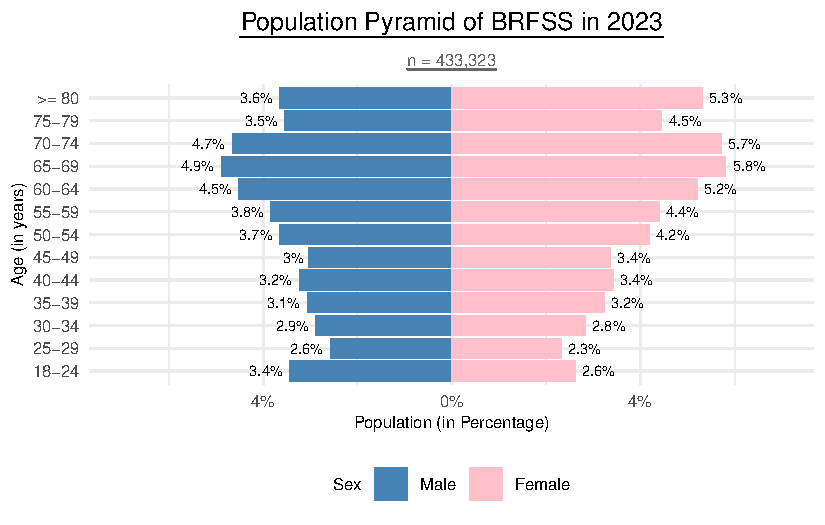
\includegraphics{Report_Diabetes_Behavioral_Factors_Analysis_files/figure-pdf/unnamed-chunk-17-1.pdf}

Interpretation:

\begin{enumerate}
\def\labelenumi{\arabic{enumi}.}
\setcounter{enumi}{1}
\tightlist
\item
  Biological Characteristics:
\end{enumerate}

\begin{Shaded}
\begin{Highlighting}[]
\FunctionTok{summary}\NormalTok{(df}\SpecialCharTok{$}\NormalTok{BMI, }\AttributeTok{na.rm =} \ConstantTok{TRUE}\NormalTok{)}
\end{Highlighting}
\end{Shaded}

\begin{verbatim}
   Min. 1st Qu.  Median    Mean 3rd Qu.    Max.    NA's 
  12.02   24.10   27.40   28.48   31.62   99.84   40535 
\end{verbatim}

Interpretation: Mean BMI of the respondents is 28.5, stating, in
average, respondent were overweight.

\begin{enumerate}
\def\labelenumi{\arabic{enumi}.}
\setcounter{enumi}{2}
\tightlist
\item
  Behavioral Characteristics: 3.1 Grouped bar-plot for
  physical\_activity, smoking, tobacco\_use, alc\_drnk\_30days
\end{enumerate}

\begin{Shaded}
\begin{Highlighting}[]
\NormalTok{behav\_char }\OtherTok{\textless{}{-}}\NormalTok{ df[}\FunctionTok{c}\NormalTok{(}\StringTok{"physical\_activity"}\NormalTok{, }
                   \StringTok{"smoking"}\NormalTok{, }
                   \StringTok{"tobacco\_use"}\NormalTok{, }
                   \StringTok{"alc\_drnk\_30days"}\NormalTok{)]}

\CommentTok{\# Removing NAs from all to make plots comparable}
\NormalTok{behav\_char\_clean }\OtherTok{\textless{}{-}}\NormalTok{ behav\_char[}\FunctionTok{complete.cases}\NormalTok{(behav\_char), ]}

\CommentTok{\# Count observation for n}
\CommentTok{\# nrow(behav\_char\_clean)}

\CommentTok{\# Counts table}
\NormalTok{tab\_behav }\OtherTok{\textless{}{-}} \FunctionTok{sapply}\NormalTok{(behav\_char\_clean, table)}

\CommentTok{\# Transpose to wide data frame}
\NormalTok{l\_tab\_behav }\OtherTok{\textless{}{-}} \FunctionTok{as.data.frame}\NormalTok{(}\FunctionTok{t}\NormalTok{(tab\_behav))}
\NormalTok{l\_tab\_behav}\SpecialCharTok{$}\NormalTok{variable }\OtherTok{\textless{}{-}} \FunctionTok{rownames}\NormalTok{(l\_tab\_behav)}

\CommentTok{\# Reshape to long}
\NormalTok{counts\_long }\OtherTok{\textless{}{-}} \FunctionTok{reshape}\NormalTok{(l\_tab\_behav,}
                       \AttributeTok{varying   =} \FunctionTok{c}\NormalTok{(}\StringTok{"Yes"}\NormalTok{, }\StringTok{"No"}\NormalTok{),}
                       \AttributeTok{v.names   =} \StringTok{"Count"}\NormalTok{,}
                       \AttributeTok{timevar   =} \StringTok{"Response"}\NormalTok{,}
                       \AttributeTok{times     =} \FunctionTok{c}\NormalTok{(}\StringTok{"Yes"}\NormalTok{, }\StringTok{"No"}\NormalTok{),}
                       \AttributeTok{direction =} \StringTok{"long"}\NormalTok{)}
\CommentTok{\# Set factor orders}
\NormalTok{counts\_long}\SpecialCharTok{$}\NormalTok{Response }\OtherTok{\textless{}{-}} \FunctionTok{factor}\NormalTok{(counts\_long}\SpecialCharTok{$}\NormalTok{Response, }\AttributeTok{levels =} \FunctionTok{c}\NormalTok{(}\StringTok{"Yes"}\NormalTok{, }\StringTok{"No"}\NormalTok{))}
\NormalTok{counts\_long}\SpecialCharTok{$}\NormalTok{variable }\OtherTok{\textless{}{-}} \FunctionTok{factor}\NormalTok{(counts\_long}\SpecialCharTok{$}\NormalTok{variable,}
                               \AttributeTok{levels =} \FunctionTok{c}\NormalTok{(}\StringTok{"physical\_activity"}\NormalTok{, }\StringTok{"smoking"}\NormalTok{,}
                                          \StringTok{"tobacco\_use"}\NormalTok{, }\StringTok{"alc\_drnk\_30days"}\NormalTok{),}
                               \AttributeTok{labels =} \FunctionTok{c}\NormalTok{(}\StringTok{"Physical activity"}\NormalTok{, }\StringTok{"Smoking"}\NormalTok{,}
                                          \StringTok{"Tobacco use"}\NormalTok{, }\StringTok{"Alc 30days"}\NormalTok{))}
\CommentTok{\# Bar plot}
\FunctionTok{ggplot}\NormalTok{(counts\_long, }\FunctionTok{aes}\NormalTok{(}\AttributeTok{x =}\NormalTok{ Response, }\AttributeTok{y =}\NormalTok{ Count, }\AttributeTok{fill =}\NormalTok{ Response)) }\SpecialCharTok{+}
  \FunctionTok{geom\_bar}\NormalTok{(}\AttributeTok{stat =} \StringTok{"identity"}\NormalTok{, }\AttributeTok{width =} \FloatTok{0.6}\NormalTok{) }\SpecialCharTok{+}
  \FunctionTok{scale\_fill\_manual}\NormalTok{(}\AttributeTok{values =} \FunctionTok{c}\NormalTok{(}\StringTok{"Yes"} \OtherTok{=} \StringTok{"\#1f77b4"}\NormalTok{, }\StringTok{"No"} \OtherTok{=} \StringTok{"orange"}\NormalTok{)) }\SpecialCharTok{+}
  \FunctionTok{scale\_y\_continuous}\NormalTok{(}\AttributeTok{labels =}\NormalTok{ scales}\SpecialCharTok{::}\NormalTok{comma, }\AttributeTok{expand =} \FunctionTok{expansion}\NormalTok{(}\AttributeTok{mult =} \FunctionTok{c}\NormalTok{(}\DecValTok{0}\NormalTok{, }\FloatTok{0.12}\NormalTok{))) }\SpecialCharTok{+}
  \FunctionTok{facet\_wrap}\NormalTok{(}\SpecialCharTok{\textasciitilde{}}\NormalTok{ variable, }\AttributeTok{nrow =} \DecValTok{2}\NormalTok{, }\AttributeTok{ncol =} \DecValTok{2}\NormalTok{) }\SpecialCharTok{+}
  \FunctionTok{geom\_text}\NormalTok{(}\FunctionTok{aes}\NormalTok{(}\AttributeTok{label =}\NormalTok{ scales}\SpecialCharTok{::}\FunctionTok{comma}\NormalTok{(Count)),}
            \AttributeTok{vjust =} \SpecialCharTok{{-}}\FloatTok{0.4}\NormalTok{, }\AttributeTok{size =} \FloatTok{3.2}\NormalTok{) }\SpecialCharTok{+}
  \FunctionTok{labs}\NormalTok{(}\AttributeTok{title =} \FunctionTok{expression}\NormalTok{(}\FunctionTok{underline}\NormalTok{(}\StringTok{"Behavioral Characteristics"}\NormalTok{)),}
       \AttributeTok{subtitle =} \FunctionTok{expression}\NormalTok{(}\FunctionTok{underline}\NormalTok{(}\StringTok{"n = 399,230"}\NormalTok{)),}
       \AttributeTok{x =} \ConstantTok{NULL}\NormalTok{, }\AttributeTok{y =} \StringTok{"Count"}\NormalTok{) }\SpecialCharTok{+}
  \FunctionTok{theme\_minimal}\NormalTok{(}\AttributeTok{base\_size =} \DecValTok{12}\NormalTok{) }\SpecialCharTok{+}
  \FunctionTok{theme}\NormalTok{(}
        \AttributeTok{plot.title =} \FunctionTok{element\_text}\NormalTok{(}\AttributeTok{hjust =} \FloatTok{0.5}\NormalTok{, }
                                   \AttributeTok{size =} \DecValTok{12}\NormalTok{),}
        \AttributeTok{plot.subtitle =} \FunctionTok{element\_text}\NormalTok{(}\AttributeTok{hjust =} \FloatTok{0.5}\NormalTok{,}
                                  \AttributeTok{size =} \DecValTok{8}\NormalTok{, }
                                 \AttributeTok{color =} \StringTok{"gray40"}\NormalTok{),}
        \AttributeTok{axis.title =} \FunctionTok{element\_text}\NormalTok{(}\AttributeTok{size =} \DecValTok{8}\NormalTok{),}
        \AttributeTok{axis.text =} \FunctionTok{element\_text}\NormalTok{(}\AttributeTok{size =} \DecValTok{8}\NormalTok{, }
                                \AttributeTok{hjust =} \DecValTok{1}\NormalTok{),}
        \AttributeTok{legend.position    =} \StringTok{"none"}\NormalTok{,}
        \AttributeTok{strip.text         =} \FunctionTok{element\_text}\NormalTok{(}\AttributeTok{face =} \StringTok{"bold"}\NormalTok{),}
        \AttributeTok{panel.grid.major.x =} \FunctionTok{element\_blank}\NormalTok{())}
\end{Highlighting}
\end{Shaded}

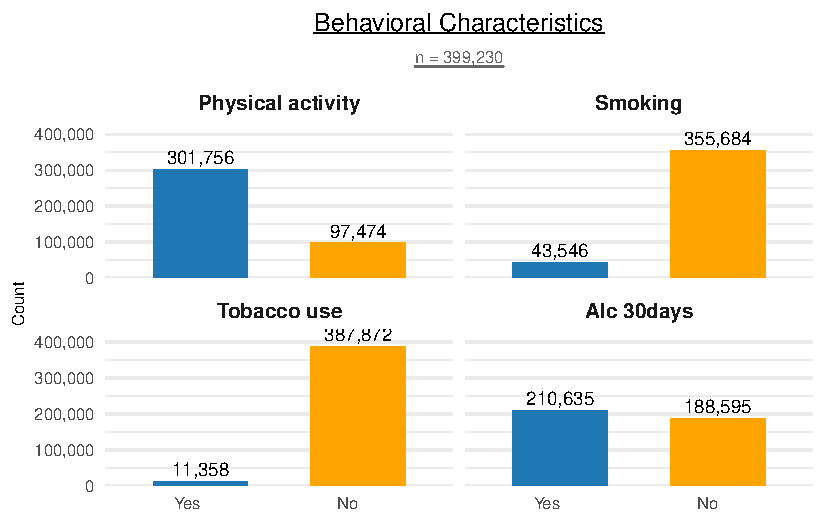
\includegraphics{Report_Diabetes_Behavioral_Factors_Analysis_files/figure-pdf/unnamed-chunk-19-1.pdf}

Interpretation:

\begin{enumerate}
\def\labelenumi{\arabic{enumi}.}
\setcounter{enumi}{3}
\tightlist
\item
  Diabetes related: 4.1 Diabetes Status by Income Level
\end{enumerate}

\begin{Shaded}
\begin{Highlighting}[]
\FunctionTok{ggplot}\NormalTok{(income\_diab\_clean, }\FunctionTok{aes}\NormalTok{(}\AttributeTok{x =}\NormalTok{ income\_level, }\AttributeTok{fill =}\NormalTok{ diabetes\_status)) }\SpecialCharTok{+}
  \FunctionTok{geom\_bar}\NormalTok{(}\AttributeTok{position =} \StringTok{"dodge"}\NormalTok{) }\SpecialCharTok{+}
  \FunctionTok{scale\_fill\_manual}\NormalTok{(}\AttributeTok{values =} \FunctionTok{c}\NormalTok{(}\StringTok{"Yes"} \OtherTok{=} \StringTok{"darkred"}\NormalTok{, }\StringTok{"No"} \OtherTok{=} \StringTok{"\#4daf4a"}\NormalTok{)) }\SpecialCharTok{+}
  \FunctionTok{labs}\NormalTok{(}
    \AttributeTok{title =} \FunctionTok{expression}\NormalTok{(}\FunctionTok{underline}\NormalTok{(}\StringTok{"Diabetes Status by Income Level"}\NormalTok{)),}
    \AttributeTok{subtitle =} \FunctionTok{expression}\NormalTok{(}\FunctionTok{underline}\NormalTok{(}\StringTok{"n = 346,224"}\NormalTok{)),}
    \AttributeTok{x =} \StringTok{"Income Level"}\NormalTok{,}
    \AttributeTok{y =} \StringTok{"Frequency"}\NormalTok{,}
    \AttributeTok{fill =} \StringTok{"Diabetes"}
\NormalTok{  ) }\SpecialCharTok{+}
  \FunctionTok{theme\_minimal}\NormalTok{() }\SpecialCharTok{+}
  \FunctionTok{theme}\NormalTok{(}
    \AttributeTok{plot.title =} \FunctionTok{element\_text}\NormalTok{(}\AttributeTok{hjust =} \FloatTok{0.5}\NormalTok{, }
                              \AttributeTok{size =} \DecValTok{12}\NormalTok{),}
    \AttributeTok{axis.title =} \FunctionTok{element\_text}\NormalTok{(}\AttributeTok{size =} \DecValTok{8}\NormalTok{),}
    \AttributeTok{plot.subtitle =} \FunctionTok{element\_text}\NormalTok{(}\AttributeTok{hjust =} \FloatTok{0.5}\NormalTok{,}
                                  \AttributeTok{size =} \DecValTok{8}\NormalTok{, }
                                 \AttributeTok{color =} \StringTok{"gray40"}\NormalTok{),}
    \AttributeTok{axis.line =} \FunctionTok{element\_line}\NormalTok{(}\AttributeTok{color =} \StringTok{"grey"}\NormalTok{, }
                          \AttributeTok{linewidth =} \FloatTok{0.8}\NormalTok{),}
    \AttributeTok{axis.text =} \FunctionTok{element\_text}\NormalTok{(}\AttributeTok{size =} \DecValTok{8}\NormalTok{, }
                            \AttributeTok{angle =} \DecValTok{45}\NormalTok{,}
                            \AttributeTok{hjust =} \DecValTok{1}\NormalTok{))}
\end{Highlighting}
\end{Shaded}

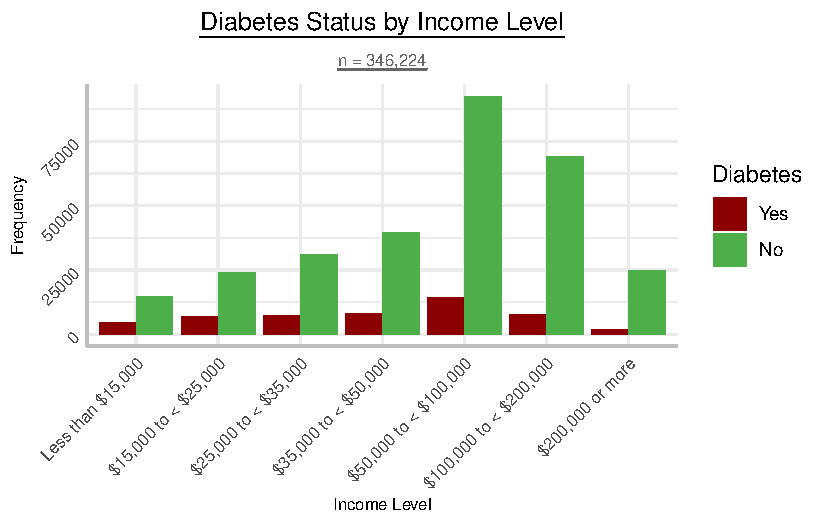
\includegraphics{Report_Diabetes_Behavioral_Factors_Analysis_files/figure-pdf/unnamed-chunk-21-1.pdf}

Interpretation:

4.2 US States by Diabetes Prevalence: BRFSS, 2023

\begin{Shaded}
\begin{Highlighting}[]
\CommentTok{\# Visualize the diabetes prevalence on US MAP}
\CommentTok{\# Create dataframe with state name and diabetes cases}
\NormalTok{diab\_st\_df }\OtherTok{\textless{}{-}} \FunctionTok{as.data.frame}\NormalTok{(}\FunctionTok{table}\NormalTok{(df}\SpecialCharTok{$}\NormalTok{state\_name, df}\SpecialCharTok{$}\NormalTok{diabetes\_status))}
\FunctionTok{colnames}\NormalTok{(diab\_st\_df) }\OtherTok{\textless{}{-}} \FunctionTok{c}\NormalTok{(}\StringTok{"state"}\NormalTok{, }
                     \StringTok{"diabetes\_status"}\NormalTok{, }
                     \StringTok{"frequency"}\NormalTok{)}

\CommentTok{\# Widening the df with separate "No" count}
\NormalTok{diab\_st\_df }\OtherTok{\textless{}{-}} \FunctionTok{reshape}\NormalTok{(diab\_st\_df, }
                     \AttributeTok{idvar =} \FunctionTok{names}\NormalTok{(diab\_st\_df)[}\DecValTok{1}\NormalTok{],}
                     \AttributeTok{timevar =} \StringTok{"diabetes\_status"}\NormalTok{, }
                     \AttributeTok{direction =} \StringTok{"wide"}\NormalTok{,}
                     \AttributeTok{v.names =} \StringTok{"frequency"}\NormalTok{)}
\FunctionTok{names}\NormalTok{(diab\_st\_df) }\OtherTok{\textless{}{-}} \FunctionTok{gsub}\NormalTok{(}\StringTok{"frequency}\SpecialCharTok{\textbackslash{}\textbackslash{}}\StringTok{."}\NormalTok{, }\StringTok{""}\NormalTok{, }\FunctionTok{names}\NormalTok{(diab\_st\_df))}
\NormalTok{diab\_st\_df}\SpecialCharTok{$}\NormalTok{total }\OtherTok{\textless{}{-}}\NormalTok{ diab\_st\_df}\SpecialCharTok{$}\NormalTok{Yes }\SpecialCharTok{+}\NormalTok{ diab\_st\_df}\SpecialCharTok{$}\NormalTok{No}

\NormalTok{diab\_st\_df}\SpecialCharTok{$}\NormalTok{prevalence }\OtherTok{\textless{}{-}}\NormalTok{ (diab\_st\_df}\SpecialCharTok{$}\NormalTok{Yes }\SpecialCharTok{/}\NormalTok{ diab\_st\_df}\SpecialCharTok{$}\NormalTok{total) }\SpecialCharTok{*} \DecValTok{100}

\CommentTok{\# Before plotting, verify all U.S. states are represented in diab\_state\_df}
\CommentTok{\# by comparing against the built{-}in \textquotesingle{}statepop\textquotesingle{} reference dataset from the}
\CommentTok{\# usmap package.}

\CommentTok{\# statepop \textless{}{-} usmap::statepop}
\CommentTok{\# setdiff(statepop$full, diab\_st\_df$state)}
\CommentTok{\# There is no diabetes data available from the "Kentucky", "Pennsylvania" state.}
\CommentTok{\# Sometimes the data are not reported for certain states if they don\textquotesingle{}t fulfill }
\CommentTok{\# certain requirements.}

\CommentTok{\# Prep to add each state name to label on map}

\CommentTok{\# Plotting the diabetes cases from survey in the US map}
\FunctionTok{plot\_usmap}\NormalTok{(}\AttributeTok{data =}\NormalTok{ diab\_st\_df,}
           \AttributeTok{regions =} \StringTok{"states"}\NormalTok{,}
           \AttributeTok{values =} \StringTok{"prevalence"}\NormalTok{,}
           \AttributeTok{include =} \FunctionTok{c}\NormalTok{(state.abb, }\StringTok{"PR"}\NormalTok{), }\CommentTok{\#default: excludes Puerto Rico}
           \AttributeTok{color =} \StringTok{"white"}\NormalTok{,}
           \AttributeTok{labels =} \ConstantTok{TRUE}\NormalTok{) }\SpecialCharTok{+}  
  \FunctionTok{scale\_fill\_continuous}\NormalTok{(}\AttributeTok{low =} \StringTok{"lightyellow"}\NormalTok{, }\AttributeTok{high =} \StringTok{"darkred"}\NormalTok{) }\SpecialCharTok{+}
  \FunctionTok{labs}\NormalTok{(}
    \AttributeTok{title =} \FunctionTok{expression}\NormalTok{(}\FunctionTok{underline}\NormalTok{(}\StringTok{"US States by Diabetes Prevalence: BRFSS, 2023"}\NormalTok{)),}
    \AttributeTok{subtitle =} \FunctionTok{expression}\NormalTok{(}\FunctionTok{underline}\NormalTok{(}\StringTok{"n = 433,323"}\NormalTok{)),}
    \AttributeTok{fill =} \StringTok{"Prevalence"}\NormalTok{) }\SpecialCharTok{+}
  \FunctionTok{theme}\NormalTok{(}
    \AttributeTok{plot.title =} \FunctionTok{element\_text}\NormalTok{(}\AttributeTok{hjust =} \FloatTok{0.5}\NormalTok{, }\AttributeTok{size =} \DecValTok{15}\NormalTok{, }\AttributeTok{face =} \StringTok{"bold"}\NormalTok{,}
                              \AttributeTok{margin =} \FunctionTok{margin}\NormalTok{ (}\AttributeTok{b =} \DecValTok{5}\NormalTok{)),}
    \AttributeTok{plot.subtitle =} \FunctionTok{element\_text}\NormalTok{(}\AttributeTok{hjust =} \FloatTok{0.5}\NormalTok{,}
                                  \AttributeTok{size =} \DecValTok{8}\NormalTok{, }
                                 \AttributeTok{color =} \StringTok{"black"}\NormalTok{),}
    \AttributeTok{plot.margin =} \FunctionTok{margin}\NormalTok{(}\AttributeTok{t =} \DecValTok{10}\NormalTok{, }\AttributeTok{r =} \DecValTok{10}\NormalTok{, }\AttributeTok{b =} \DecValTok{10}\NormalTok{, }\AttributeTok{l =} \DecValTok{40}\NormalTok{),}
    \AttributeTok{plot.background =} \FunctionTok{element\_rect}\NormalTok{(}\AttributeTok{fill =} \StringTok{"lightblue"}\NormalTok{, }\AttributeTok{color =} \ConstantTok{NA}\NormalTok{),}
    \AttributeTok{legend.position =} \StringTok{"right"}\NormalTok{,}
    \AttributeTok{legend.background =} \FunctionTok{element\_rect}\NormalTok{(}\AttributeTok{fill =} \StringTok{"lightblue"}\NormalTok{, }\AttributeTok{color =} \ConstantTok{NA}\NormalTok{))}
\end{Highlighting}
\end{Shaded}

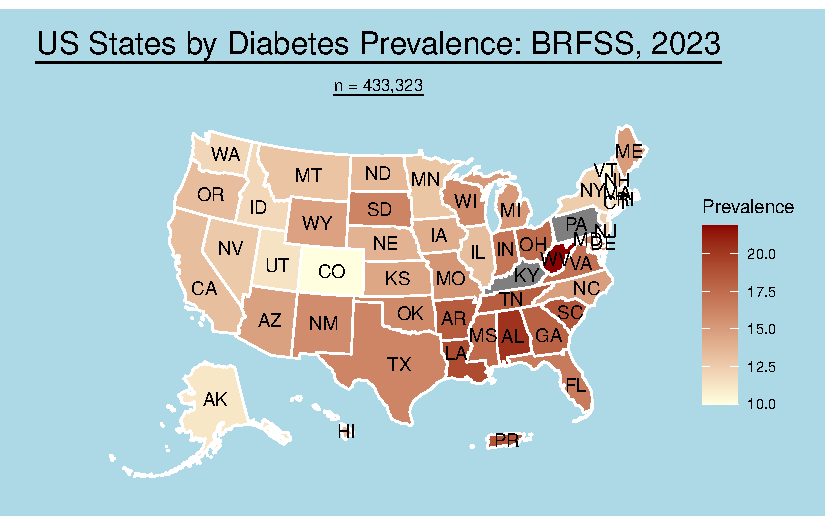
\includegraphics{Report_Diabetes_Behavioral_Factors_Analysis_files/figure-pdf/unnamed-chunk-22-1.pdf}

Interpretation: West Virginie had highest prevalence of diabetes in year
2023.

4.3 Mean Age of First Known Diabetes Diagnosis

\begin{Shaded}
\begin{Highlighting}[]
\NormalTok{mean\_diab\_first }\OtherTok{\textless{}{-}} \FunctionTok{mean}\NormalTok{(df}\SpecialCharTok{$}\NormalTok{diab\_first\_known, }\AttributeTok{na.rm =} \ConstantTok{TRUE}\NormalTok{)}
\end{Highlighting}
\end{Shaded}

Interpretation: On average, individuals in this dataset first became
aware of their diabetes diagnosis at approximately 53.40 years of age.

\subsection{Multivariable Logistic Regression
Analysis}\label{multivariable-logistic-regression-analysis}

Since we are interested to test the association of behavioral variables
with the Diabetes, only relevant variables were administered to the
model. Further, logistic regression predicts the probability of the
higher level, hence, for better interpretation of the results, the level
were reordered as ``no'' and ``yes''.

\begin{Shaded}
\begin{Highlighting}[]
\CommentTok{\# Logistics regression calculation}
\NormalTok{LR\_1 }\OtherTok{\textless{}{-}} \FunctionTok{glm}\NormalTok{(diabetes\_status }\SpecialCharTok{\textasciitilde{}}\NormalTok{ physical\_activity }\SpecialCharTok{+}\NormalTok{ smoking }\SpecialCharTok{+}\NormalTok{ tobacco\_use }\SpecialCharTok{+}
\NormalTok{              alc\_drnk\_30days, }
            \AttributeTok{family =} \FunctionTok{binomial}\NormalTok{(}\AttributeTok{link =} \StringTok{"logit"}\NormalTok{), }\AttributeTok{data =}\NormalTok{ df)}

\CommentTok{\# Report estimated odds ratio,p{-}value and 95\% CI. }
\NormalTok{jtools}\SpecialCharTok{::}\FunctionTok{summ}\NormalTok{(LR\_1, }\AttributeTok{exp =}\NormalTok{ T, }\AttributeTok{confint =}\NormalTok{ T, }\AttributeTok{model.fit =}\NormalTok{ F, }\AttributeTok{digits =} \DecValTok{3}\NormalTok{)}
\end{Highlighting}
\end{Shaded}

\begin{table}[!h]
\centering
\begin{tabular}{lr}
\toprule
\cellcolor{gray!10}{Observations} & \cellcolor{gray!10}{398508 (34815 missing obs. deleted)}\\
Dependent variable & diabetes\_status\\
\cellcolor{gray!10}{Type} & \cellcolor{gray!10}{Generalized linear model}\\
Family & binomial\\
\cellcolor{gray!10}{Link} & \cellcolor{gray!10}{logit}\\
\bottomrule
\end{tabular}
\end{table}  \begin{table}[!h]
\centering
\begin{threeparttable}
\begin{tabular}{lrrrrr}
\toprule
  & exp(Est.) & 2.5\% & 97.5\% & z val. & p\\
\midrule
\cellcolor{gray!10}{(Intercept)} & \cellcolor{gray!10}{0.089} & \cellcolor{gray!10}{0.084} & \cellcolor{gray!10}{0.095} & \cellcolor{gray!10}{-79.455} & \cellcolor{gray!10}{0.000}\\
physical\_activityNo & 2.035 & 1.996 & 2.074 & 73.328 & 0.000\\
\cellcolor{gray!10}{smokingNo} & \cellcolor{gray!10}{1.097} & \cellcolor{gray!10}{1.066} & \cellcolor{gray!10}{1.129} & \cellcolor{gray!10}{6.283} & \cellcolor{gray!10}{0.000}\\
tobacco\_useNo & 0.981 & 0.929 & 1.037 & -0.671 & 0.502\\
\cellcolor{gray!10}{alc\_drnk\_30daysNo} & \cellcolor{gray!10}{2.015} & \cellcolor{gray!10}{1.978} & \cellcolor{gray!10}{2.053} & \cellcolor{gray!10}{74.048} & \cellcolor{gray!10}{0.000}\\
\bottomrule
\end{tabular}
\begin{tablenotes}
\item Standard errors: MLE
\end{tablenotes}
\end{threeparttable}
\end{table}

Interpretation: According to multivariable logistic regression, the odds
of having diabetes among those who are not physically active in a month
increases by 2.035 times (95\% CI:1.996 to 2.074; p-value \textless{}
0.001). Similarly, the odds of having diabetes among those who drink
alcohol in 30 days increases by 2.015 times (95\% CI: 1.978 to 2.053;
p-value \textless{} 0.001). Interestingly, model showed that current
non-smokers had statistically significant likelihood of having diabetes
by 1.097 times (95\% CI: 1.066 to 1.129; p-value \textless{} 0.001)
compared to those who did not smoke. However, there is no statistical
significant association of current tobacco use with having diabetes OR =
0.981 (95\% CI: 0.929 to 1.037; p-value = 0.502). In conclusion, only
``Physical Activity in a month'' and ``Alcohol Consumption in 30 days''
among the behavioral characteristics, have statistical significant
association with the diabetes.




\end{document}
